
%%%%%%%%%%%%%%%%%%%%%%%%%%%%%%%%%%%%%%%%%%%%%%%%%%%%%%%%%%%%%%%%%%%%%%%%%%%%%
\chapt[chap:mimir]{GATE \Mimir}
\markboth{GATE \Mimir}{GATE \Mimir}
%%%%%%%%%%%%%%%%%%%%%%%%%%%%%%%%%%%%%%%%%%%%%%%%%%%%%%%%%%%%%%%%%%%%%%%%%%%%%
\nnormalsize


%%%%%%%%%%%%%%%%%%%%%%%%%%%%%%%%%%%%%%%
%\sect[sec:family:mimir]{GATE MIMIR}

\Mimir\ \footnote{Old Norse \textit{``The rememberer, the wise one''.}} 
is a multi-paradigm information management index and repository which
can be used to index and search over text, annotations, semantic schemas
(ontologies), and semantic meta-data (instance data). It allows queries that
arbitrarily mix full-text, structural, linguistic and semantic queries and that
can scale to terabytes of text.

\ifprintedbook
This chapter provides an overview of \Mimir\ and its functionalities. For a 
complete user guide, including code samples, please see 
\htlinkplain{http://gate.ac.uk/family/mimir.html}.

\section{What Is in a \Mimir\ Index?}

A typical semantic annotation project deals with large quantities of data of
different kinds. \Mimir\ provides a framework for implementing indexing and
search functionality across all these data types, listed below in the order of
increasing information density:

{\bf Text}\\
All documents have a textual content. Support for full text search represents
the most basic indexing functionality and it is required in most (if not all)
cases.  Even when semantic annotation is used to abstract away from the
actual textual data, the original content still needs to be accessible so
that it can be used to provide textual query fragments in the case of more
complex conceptual queries.

\Mimir\ uses inverted indexes\footnote{{\em Inverted Indexes} are data
structures traditionally used in Information Retrieval to support indexing of
text.} for indexing the document content (including additional linguistic
information, such as part-of-speech or morphological roots), and for
associating instance of annotations with the position in the input text where
they occur. The inverted index implementation used by \Mimir\ is based on
MG4J\footnote{\url{http://mg4j.dsi.unimi.it/}}.

{\bf Annotations}\\
The first step in abstracting away from the plain text content is the
production of {\em annotations}. Annotations are meta-data associated to text
snippets in the documents. \Mimir's view of annotations is based on that of
GATE, with each annotation described by
\begin{itemize}
  \item the document it belongs to;
  \item the start and end offset of the referred text snippet;
  \item the annotation type;
  \item an arbitrary set of \verb!<!feature,value\verb!>! pairs.
\end{itemize}

An annotation index supports a more generic search paradigm. Depending on the
type of annotations available, the user can search across different dimensions.
If, for example, the documents are annotated with occurrences of {\tt Person,
Location, Organization} entities, then searches like {\tt \{Person\}, CEO of
\{Organization\}, based in \{Location\}} become possible.  Storage of
annotation data in \Mimir\ indexes is handled by plugins, \Mimir\ ships with
two storage plugins by default, one storing annotation data in a relational
database and the other in a Knowledge Base to support richer semantic querying.

ANNIC (ANNotations In
Context) (see Chapter~\ref{chap:annic}) is a tool
predating \Mimir\ that supports the indexing of annotations, and that has been
used to inform the design of \Mimir.

{\bf Knowledge Base Data}\\
Knowledge Base (KB) Data  consists of an ontology populated with instances. The
ontology represents the data schema and comprises a hierarchy of class types
and a hierarchy of properties that are applicable between instances of classes.
The instance data represents facts that are known to the systems and is
typically at least partially derived from semantic annotation over documents.
KB data is used to reach a higher level of abstraction over the information in
the documents which enables conceptual queries such as ``find all mentions of
{\tt Person}s who are employed by any organization based in Yorkshire''.

A KB that is pre-populated with appropriate world knowledge can perform other
generalisations that are natural to humans users, such as being able to identify
Vienna as a valid answer to queries relating to Austria, Europe or the Western
Hemisphere.

As mentioned above, \Mimir\ can make use of a Knowledge Base to store
information relating to annotations. The links between annotations, the textual
data, and the knowledge base information are created by the inclusion into the
text indexes of a set specially-created URIs that are associated with
annotation data. Furthermore, URIs of entities from the Knowledge Base can be
stored as annotation features.

Knowledge bases are typically represented as a collection of triples that are
kept in highly-specialised and optimised triple stores, using standards such as
RDF or one the versions of OWL\footnote{See
\url{http://www.w3.org/RDF/} and \url{http://www.w3.org/TR/owl-features/}.}. The
implementation used by \Mimir\ is based on ORDI and
OWLIM\footnote{See
\url{http://www.ontotext.com/ordi/} and \url{http://www.ontotext.com/owlim/}.}.

%%%%%%%%%%%%%%%%%%%%%%%%%%%%%%%%%%%%%%%%%%%%%%%%%%%%%%%%%%%%%
\section{Types of Indexes}\label{sec:mimir:index-types}
%%%%%%%%%%%%%%%%%%%%%%%%%%%%%%%%%%%%%%%%%%%%%%%%%%%%%%%%%%%%%

A single instance of \Mimir\ can host several indexes.  \Mimir\ supports
{\em local} indexes, stored in the file system of the \Mimir\ server, and
{\em remote} indexes, which are a view of an index hosted in another \Mimir\
instance (possibly on a different machine).  Several indexes (of any type) can
be combined into a {\em federated} index, which presents the group of indexes as
a single virtual index.  All the indexing and searching functionality of
\Mimir\ applies equally to all three index types.

Each \Mimir\ index has a {\em state}, and the operations that can be performed
on the index depend on which state it is currently in.  When first created, a
local index will be in the {\em indexing} state, meaning it is waiting for
documents to be added to the index.  When all the documents have been added to
the index an administrator will close the index, putting it into the {\em
closing} state.  For large indexes the closing process can take several hours,
and when it is complete the index will enter the {\em searching} state, at
which point it is available for querying.  The other possible state for a local
index is {\em failed}, indicating a problem with the index.  Typically a failed
index will need to be deleted by the administrator.  Thus it is apparent that
an index cannot be used simultaneously for searching and indexing.  An existing
set of index files can be imported into a running \Mimir\ instance as a local
index, which will then immediately be in the {\em searching} state.

Remote indexes inherit their state from the remote server, and federated
indexes inherit their state by combining the states of their component indexes.
A federated index may occasionally appear in the {\em working} state if its
component indexes are not all in the same state (for example if some of them
have started closing but others are still in {\em indexing} mode), but the
working state will usually resolve to a normal state once the component indexes
have synchronized.

Note that once a local index has moved from {\em indexing} to {\em closing} to
{\em searching} it is not possible to add more documents to the same index.
The suggested way to add to an index is to create a new index to hold the new
documents, fill it, close it, and then create a federated index consisting of
the original index plus the new one (or if the original index was itself
federated, add the new index to the existing federation).

A typical setup for a large-scale indexing task would be to have a number of
identical ``slave'' servers running \Mimir, each with a single local index.  A
single ``master'' \Mimir\ instance could then have one remote index definition
pointing to each of the slaves, and a single federated index combining the
remote indexes.  This federated index would be the point of entry into the
system and would share out indexing jobs (round-robin among the slaves) or
search requests (to all the slaves in parallel) as appropriate.

Due to space limitations, we refer the reader to the 
\htlink{http://gate.ac.uk/family/mimir.html}{\Mimir\ User Guide} for 
details on how to setup \Mimir\ and manage the different types of indexes.


%%%%%%%%%%%%%%%%%%%%%%%%%%%%%%%%%%%%%%%%%%%%%%%%%%%%%%%%%%%%%%%%%%%%%%%%%%
\section{Searching \Mimir\ Indexes}\label{sec:mimir:searching}
%%%%%%%%%%%%%%%%%%%%%%%%%%%%%%%%%%%%%%%%%%%%%%%%%%%%%%%%%%%%%%%%%%%%%%%%%%

From a user's point of view, \Mimir\ is a tool for searching a collection of
semantically annotated documents.  It provides facilities for searching over
different views of the document text, for example one can search the document
words, the part-of-speech of those words, or their morphological roots. Beside
searching the document text, \Mimir\ also supports searches over the documents'
semantic annotations, where queries are based on annotation types and
restrictions over the values of annotation features. These different search
paradigms can be combined freely into complex queries, with support for
sequences, repetitions, and Boolean operators.

A search session entails the formulation of a query, running the query with the
\Mimir\ query engine, and consuming the query results.  \Mimir\ queries are
expressed in a text-based query language which is described in
section~\ref{sec:mimir-search:ql}.  The way these queries are submitted to \Mimir\
depends on how it is deployed, the various interfaces are discussed in
section~\ref{sec:mimir-search:interfaces}.


\section{The \Mimir\ Query Language}\label{sec:mimir-search:ql}

A \Mimir\ query is either a simple query (i.e. a {\tt String} query,
or an {\tt Annotation} query), or a compound one, 
which comprises a set of
sub-queries linked by operators. If no operator is placed between any two
sub-queries, then the {\tt Sequence} operator is implied (see below for details). 
This means that several queries
written one after another are interpreted as one sequence query. For example, a
query like `{\it the brown dog}' is interpreted as a sequence query, having
three sub-queries, each of them being a String query. This would match
occurrences of the exact phrase `{\it the brown dog}' in the indexed documents.
Note that this is different from the standard behaviour of search engines,
which would simply match documents in which all three query terms occur, in
whichever order. That type of search is also supported in \Mimir, through the
{\tt AND} operator.  
Parentheses can be used
for grouping where the syntax would otherwise be ambiguous.

\subsubsection{String Queries}\label{sec:mimir-search:string-query}

The simplest form of query is a query term. This will match all occurrences of
the query term in the indexed documents.

If the \Mimir\ index being interrogated includes multiple token indexes, then
the particular index to be searched can be specified by prefixing the query
term with the index name and a colon, for example the query
`{\it root:be}'\footnote{This assumes that an index named {\tt root} exists,
and was used to store the morphological root of the words.} will match all
morphological forms of the verb {\it to be}. If the name of the string index is
omitted, then the first configured index is used. By convention (reflected in
the default \Mimir\ configuration) the first string index is used to store the
terms text, so the default behaviour is to search over the document text, as
expected.  Double-quoted strings are treated as plain term queries against the
first token index in a similar way.

In fact the above is a slight simplification, as bare terms (and double-quoted
strings) are actually tokenised before being searched for.  This is because
\Mimir\ views documents as streams of tokens, not characters, and the query
must match the tokenisation that was used to index the documents.  For example,
the default GATE tokeniser treats ``don't'' as two tokens, ``do'' and ``n't'',
so a query for {\em don't} as a single token would fail.  To get around this,
\Mimir\ runs a GATE application over the string of the query to generate
Token annotations, and then constructs a query for these tokens in sequence.  
Named index queries (``root:be'') are
not tokenised, so if you want to avoid tokenising a particular query for any
reason (e.g. if you suspect there is a mis-tokenised document in your index)
you can explicitly name the appropriate index (typically ``string'', i.e.
string:don't).

\subsubsection{Annotation Queries}\label{sec:mimir-search:annotation-query}

If annotation indexes were used during indexing, \Mimir\ allows searching for
annotation-based patterns. An annotation is a piece of metadata
associated with a text segment, with a {\bf type} and optionally
{\bf features}.  An annotation query takes the following form: 
{\tt \{Type feature1=value1 feature2=value2 \ldots\}}.  The annotation type is
required, the feature constraints are optional.

While the example above uses equality for the feature constraints, other
operators are also available. Here is the full list:
\begin{description}
  \item[equality:] represented by the sign $=$, matches annotations which have
  the given value for the specified feature. The equality operator is
  applicable to features of any type.
  \item[comparison operators:] represented by one of the following symbols:
  $<$, $<=$, $>$, $>=$, with the usual meaning. These operators can apply to
  features of type {\tt nominal}, {\tt numeric}, or {\tt text}.
  \item[regular expressions:] can be specified using the syntax {\tt
  REGEX(pattern, flags)}, where the {\tt pattern} represents the regular
  expression sought, and the {\tt flags} are optional, and can be used to
  change the way matching is performed. See
  \url{http://www.w3.org/TR/xpath-functions/#regex-syntax} for a full
  specification of the regular expression support. The {\tt REGEX} operator can
  only be used for {\tt nominal}, and {\tt text} features.
\end{description}

Examples:\\
\{Person gender $=$ female\} -- searches for annotations of type
{\tt Person}, which have a feature named {\tt gender}, with the value
{\it female}.

\{Measurement type $=$ scalar normalisedValue $>0$ normalisedValue $<10$
normalisedUnit $=$ m\} -- searches for scalar measurements, with a unit of {\it
metre}, and a normalised value between $0$ and $10$.\footnote{The extended
support for Measurement annotations is discussed further in
the \Mimir\ User Guide.}

\subsubsection{AND Operator: ``{\tt \&}''}\label{sec:mimir-search:and-query}

The `{\tt AND}' (also `\&`) operator can be used to specify queries that should
match document segments that include at least one hit from each of the
sub-queries. The results returned will always be the shortest document segments
that satisfy the query.

\subsubsection{OR Operator: ``{\tt |}''}\label{sec:mimir-search:or-query}

{\tt OR} queries are used to search hits that match one of a set of alternative
query expressions. This is indicated by using the {\tt `OR'} (also`\verb!|!')
operator between the sub-queries. A query of the form {\tt Query1 | Query2} will
return hits that match either sub-query {\tt Query1} or sub-query {\tt Query2}.

\subsubsection{IN and OVER Operators}\label{sec:containment-query}

The operators {\tt IN} and {\tt OVER} are used to search for hits of a query
that contain, or are contained in the hits of another query. For example:
\begin{description}
\item[Query1 IN Query2] will match all the hits of {\tt Query1} that are
contained in a hit of {\tt Query2}.
\item[Query1 OVER Query2] will match all hits of {\tt Query1} that contain (are
overlapping) a hit of {\tt Query2}.
\end{description}

\subsubsection{Repeats Operator: ``+''}\label{sec:mimir-search:kleene-query}

The $+$ operator can be used to match text segments that comprise a sequence of
hits from the same sub-query. The length of the sequence is specified though a
number (representing the {\bf maximum} number of repetitions) or through two
numeric values (representing the {\bf minimum} and {\bf maximum} number of
repetitions). For example:
\begin{description}
  \item[{\tt to+3}] will match one, two, or three repeated occurrences of the
  word {\it to}. The returned hits will be of the form ``{\it to}'', ``{\it to  
  to}'', or ``{\it to to to}'').
  \item[{\tt \{Person\}+2..5}] will match sequences of 2, 3, 4, or 5
  adjacent {\tt Person} annotations.
  \item[{\tt (\{Location locType = city\} |
  \{Location locType = country\})+3}] will match any sequence of up to
  three Location annotations where each one refers to either a city or a
  country.
\end{description}

Note that there is no support for a repetition count of zero (an optional
match) -- you will need to reformulate the query to cover the versions with and
without the optional match separately and combine them with an OR, for example
{\tt (term1 term2+2 term3) | (term1 term3)}.  Similarly there is no support for
unbounded wildcards ({\em n} times or more).

\subsubsection{Sequence Queries and Gaps}\label{sec:mimir-search:sequence-query}

As sequence is the default operator in \Mimir, there is no graphical sign for
it: simply writing a set of queries one after another will cause a search for
sequences of hits, one from each sub-query. For example, the query ``{\tt the
energy level}'' is actually a sequence query where the first sub-query searches
for the word ``{\it the}'', the second for ``{\it energy}'', and the last for
``{\it level}''.

It is sometimes useful to include gaps in a sequence query, that is to allow
arbitrary text fragments (of specified length) to occur in-between the hits
from some of the sub-queries. This can be done by using the gap markers ``{\tt
[n]}'', or ``{\tt [m..n]}''. These will match a sequence of length $n$, or with
a length of between $m$ and $n$ of arbitrary tokens.

For example the query ``{\tt the [2] root:time}'' will match phrases like ``{\it
the best of times}'' or ``{\it the worst of times}'', whereas the query ``{\tt
the [2..10] root:time}'' would also match ``{\it the best use of one's time}''
(where the gap consists of six tokens -- five words and an apostrophe).

\subsubsection{Escaping Reserved Words}

Some words are part of the query language definition so they cannot be used
directly as query terms. If that is desired, then these constructs must be
escaped as shown in the following table:
\begin{center}
\begin{tabular}{|l|l|}
\hline
{\bf Reserved input} & {\bf Escaped form}\\
\hline \hline
\{, \} &  $\backslash$\{, $\backslash$\}\\
\hline
(, )  & $\backslash$(, $\backslash$) \\
\hline
[, ] & $\backslash$[, $\backslash$]\\
\hline
: &  $\backslash$: \\
\hline
+ &  $\backslash$+ \\
\hline
{\tt |} &  $\backslash${\tt |} \\
\hline
{\tt \&} &  $\backslash${\tt \&} \\
\hline
? &  $\backslash$? \\
\hline
$\backslash$ &  $\backslash$$\backslash$ \\
\hline
. &  $\backslash$. \\
\hline
" &  $\backslash$" \\
\hline 
=  & $\backslash$= \\
\hline
IN & ``IN'' \\
\hline
OVER & ``OVER''\\ 
\hline
OR & ``OR''\\ 
\hline
AND & ``AND''\\ 
\hline
\end{tabular}\\
\vspace{1ex}
Escaping reserved constructs in the \Mimir\ query language
\end{center}

\subsubsection{Semantic Queries With the {\tt ordi} Plugin}

If you are using the {\tt ordi} semantic annotation helper plugin, and have a
URI-valued feature named ``inst'' on your annotations, then the helper provides
an additional ``synthetic'' feature named {\tt semanticConstraint} that
provides a way to query for annotations based on information in the knowledge
base.
\begin{lstlisting}[breaklines]
{Organization semanticConstraint = "?inst <http://proton.semanticweb.org/2005/04/protont#locatedIn> <http://example.com#Sheffield> ."}
\end{lstlisting}

The value of the semanticConstraint feature is a SPARQL fragment that has
access to the {\tt ?inst} variable, referring to the URI in the ``inst''
feature of the annotation.  Clearly, the semanticConstraint mechanism is not
intended for direct use by end-users, but rather for use by other tools that
build \Mimir\ queries automatically.

%%%%%%%%%%%%%%%%%%%%%%%%%%%%%%%%%%%%%%%%%%%%%%%%%%%%%%%%%%%%%%%%%%%%%%%%%%

\section{Search Interfaces -- How to Submit Queries to \Mimir}
\label{sec:mimir-search:interfaces}

The \Mimir\ Grails plugin supplies two search interfaces by default, with the
infrastructure to implement other interfaces as required.  An XML-based service
interface allows other applications to submit queries to the indexes hosted by
a \Mimir\ web application by POSTing requests over HTTP (described in
section~\ref{sec:mimir-search:service}).  There is also an example user-facing search
interface called {\em GUS}, intended primarily for testing and demonstration
purposes (described in section~\ref{sec:mimir-search:gus}).  Both of these interfaces
interact with the underlying indexes through the {\tt SearchService} Grails
service provided by the plugin.  When embedding the \Mimir\ Grails plugin in
another Grails application this service is the primary means for application
code to interact with \Mimir, and is described in the \Mimir\ User Guide.

\subsection{\Mimir\ Search Web Service}\label{sec:mimir-search:service}

The \Mimir\ web application exposes the search functionality as a web service
that can be accessed through a simple HTTP interface. All requests are performed
by calling an action with a set of parameters; the results of a call are encoded
in XML and returned as the response to the request.  All the example URLs in
this section assume the {\tt demo-web-app} application with its default URL
mappings, running on {\tt localhost} port 8080.

The \Mimir\ web service can be accessed at a URL like:\\
{\tt http://localhost:8080/mimir-demo/\{index ID\}/search/\{action\}},
where the {\tt action} value is the name of one of the supported actions,
described in the \Mimir\ user guide. 
The actual URL (with the correct index ID included) can be
obtained from the {\em index information page} presented by  the \Mimir\ web
application.  Parameters may be supplied as query parameters with a {\tt GET}
request or in normal {\tt application/x-www-form-urlencoded} form in a
{\tt POST} request.  Alternatively, they may be supplied as XML (if the request
content type is {\tt text/xml} or {\tt application/xml}) of the form:
\begin{verbatim}
<request xmlns="http://gate.ac.uk/ns/mimir">
  <firstParam>value</firstParam>
  <secondParam>value</secondParam>
</request>
\end{verbatim}

The first request to the service will return a session cookie, which must be
passed back with all subsequent requests.

When accessing the service URL with no value provided for {\tt action}, a help
page will be returned presenting the documentation associated with the XML web
service.


%%%%%%%%%%%%%%%%%%%%%%%%%%%%%%%%%%%%%%%%%%%%%%%%%%%

\subsection{GUS Example User Interface}\label{sec:mimir-search:gus}

The GUS search tool is a browser-based search interface intended to serve as a
platform for experimentation with a \Mimir\ index, and as a demonstration of
the capabilities of the \Mimir\ framework and API.  It is written using the
Google Web Toolkit, and the source code is included in the \Mimir\ Grails
plugin.

In the demo web application with its default URL mappings, the GUS interface
for an index in searching mode is available at 
{\tt http://localhost:8080/mimir-demo/\{index ID\}/gus/search}.  The initial
page, shown in figure~\ref{fig:gus:front-page}, provides a text area into which
you can type queries in the \Mimir\ query language.  It provides
auto-completion for annotation types and features (by asking the index what
types it was configured with when it was created).

\begin{figure}[tbp]
\begin{center}
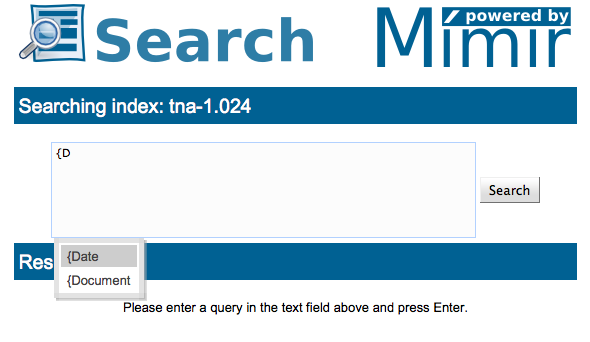
\includegraphics[scale=0.5]{gus-front-page}
\caption{Front page of the GUS user interface}
\label{fig:gus:front-page}
\end{center}
\end{figure}

Clicking the Search button starts a search on the server.  The query runs
asynchronously, collecting hits in the background until either 30 seconds have
passed or 1 million hits have been collected, at which point it stops.  To
restart the search, click the ``$>>$ keep searching'' link.

Hits are shown below the search box, as shown in figure~\ref{fig:gus:results},
with the hit text highlighted in bold and with five tokens of left and right
context.  The document title is a link, in this example to the original
document as the index was created with the ``Document URIs are external links''
option.  The ``cached'' link shows \Mimir's cached copy of the document, with
all the hits from that document highlighted in red.  For indexes where the
document URIs are not external links the document title would link directly to
the cached version and there would be no separate ``cached'' link.

\begin{figure}[tbp]
\begin{center}
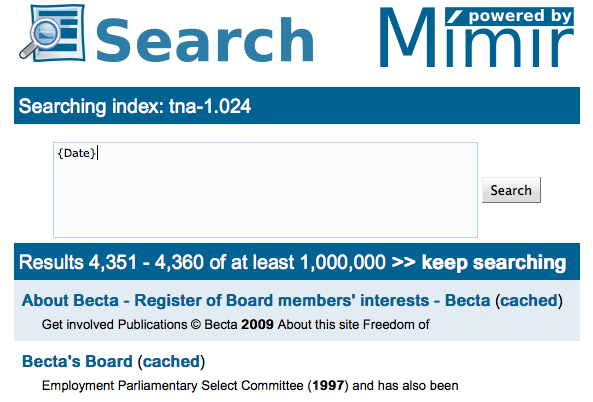
\includegraphics[scale=0.5]{gus-search-results}
\caption{GUS search results page}
\label{fig:gus:results}
\end{center}
\end{figure}

At the bottom of the page is a row of pagination links
(figure~\ref{fig:gus:pagination}).  Since, on a large index, there can be many
hundreds of thousands or even millions of hits to navigate, GUS provides links
where necessary to skip over large numbers of pages in one click.

\begin{figure}[tbp]
\begin{center}
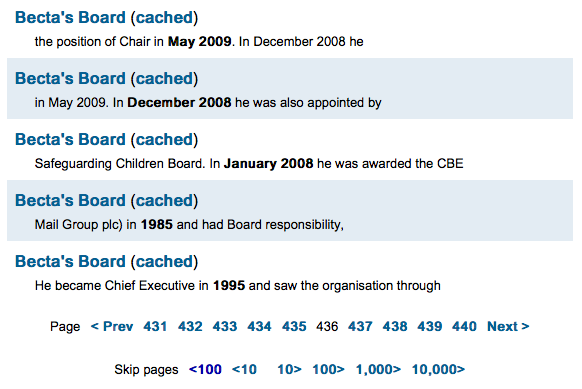
\includegraphics[scale=0.5]{gus-pagination-links}
\caption{GUS pagination links for a large search}
\label{fig:gus:pagination}
\end{center}
\end{figure}

\else % ifprintedbook

Full details on how to build and use \Mimir\ can be found in its own
\htlink{https://gate.svn.sourceforge.net/svnroot/gate/mimir/trunk/doc/mimir-guide.pdf}{user guide}.
GATE \Mimir\ is open-source software, released under the GNU Affero General
Public Licence version 3.  Commercial licences are available from the
University of Sheffield.  The source code is available from the subversion
repository at

{\tt https://gate.svn.sourceforge.net/svnroot/gate/mimir/trunk}

\fi %end of ifprintedbook
